\section{Detectors for High Energy Physics}
\label{sec:detectors}

In this section we review the basic concepts that drive the design of the LHC detectors, including ATLAS.

\subsection{Identification of Particles}

The ability to accurately identify particles and reconstruct their energy is what drives the design of detectors for high energy physics. In a detector, different sub-systems are able to capture different types of particle interaction, and the combination of the information collected by each of them allows to identify particles (or at least assign them to families, such as neutral or charged hadrons). A typical schema of the subdetectors sequence is shown in Fig. \ref{fig:detector:interaction}. The innermost layer, closer to the interaction point, is the \textit{tracking system}, dedicated to the measurement of the signed change and momentum of charged particles. The following layers are the electromagnetic and hadronic \textit{calorimeters}, that measure the energy of particles with electromagnetic and hadronic interactions respectively. The outermost layer is dedicated to the \textit{muon system}: because of their large mass (about 200 times more than electrons) muons do not produce electromagnetic showers and are therefore easy to identify as they are the only particles that reach the external part of the detector.

\begin{figure}[ht]
\centering
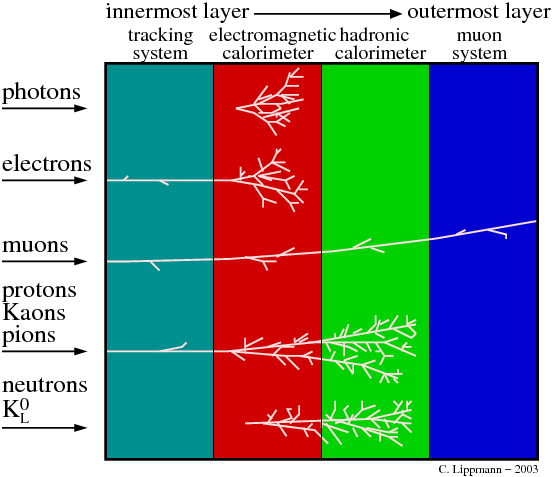
\includegraphics[width=0.6\textwidth]{figures/detector/particles_in_detector}
\caption{Components of a typical detector for physics at colliders. Different particles are identified by the distinctive signatures in the subdetectors. Figure from Ref. \cite{Lippmann:2011bb}.}
\label{fig:detector:interaction}
\end{figure}


\subsection{Tracking and Spectrometry}
A tracking device measures the traces left by charged particles passing through it. To allow the determination of the momentum and the charge of a particle, a tracking device needs to be accompanied by a magnetic field. 

\subsection{Calorimetry}

\subsubsection{Electromagnetic Cascade}

\subsubsection{Hadronic Shower}

\subsubsection{Types of Calorimeters}